\documentclass[conference]{IEEEtran}
\IEEEoverridecommandlockouts
\usepackage{cite}
\usepackage{amsmath,amssymb}
\usepackage{graphicx}
\usepackage{booktabs}
\usepackage[table]{xcolor}
\usepackage{hyperref}
\hypersetup{colorlinks=true,linkcolor=black,citecolor=black,urlcolor=black}
\definecolor{ours}{HTML}{2A78D6}
\newcommand{\best}[1]{\textbf{#1}}
\newcommand{\pmsd}[1]{{\scriptsize$\pm$#1}}
\setlength{\textfloatsep}{7pt plus 2pt minus 2pt}
\setlength{\floatsep}{6pt plus 2pt minus 2pt}
\setlength{\dbltextfloatsep}{7pt plus 2pt minus 2pt}
\setlength{\abovecaptionskip}{3pt}
\setlength{\belowcaptionskip}{0pt}

\begin{document}

\title{Monocular Geometry Priors for Endoscopic 4D Gaussian Splatting: Reproducing and Improving Endo-4DGS on StereoMIS}

\author{\IEEEauthorblockN{Author Name(s)}
\IEEEauthorblockA{Affiliation, City, Country \quad email@domain}}

\maketitle

\begin{abstract}
Endo-4DGS reconstructs deforming surgical scenes from monocular endoscopic video with 4D Gaussian splatting, using Depth-Anything to initialise and supervise geometry. We reproduce it on StereoMIS and also measure 3D accuracy against stereo depth. The released StereoMIS pipeline renders with a 34.2$^\circ$ instead of the true 58.7$^\circ$ field of view, and the metric scale of MoGe-2, a recent monocular point-map model, is 5--7$\times$ too large on endoscopic images. Correcting the intrinsics, scaling MoGe-2 with a factor triangulated from the known camera poses, and using it only to initialise the Gaussians raises PSNR from 31.98 to 32.40\,dB and lowers the rendered-depth error (AbsRel) from 0.234 to 0.148 (37\,\%), over three seeds.
\end{abstract}

\begin{IEEEkeywords}
Gaussian splatting, endoscopy, monocular depth, surgical scene reconstruction
\end{IEEEkeywords}

\section{Introduction}
Endo-4DGS~\cite{endo4dgs} models the surgical field with deformable Gaussians~\cite{kerbl3dgs,wu4dgs} whose initial point cloud and depth loss come from Depth-Anything (DA)~\cite{depthanything}; only image metrics are reported, so its 3D accuracy is unknown. We contribute (i)~a reproduction on StereoMIS~\cite{stereomis} with a geometric evaluation against stereo depth, (ii)~a fix for the field of view of the released StereoMIS preprocessing, (iii)~MoGe-2~\cite{moge2} as a geometry prior with a pose-based scale that needs no stereo, and (iv)~ablations of the depth loss, normal supervision and pose refinement, with three seeds for the main results.

\begin{figure*}[t]
\centering
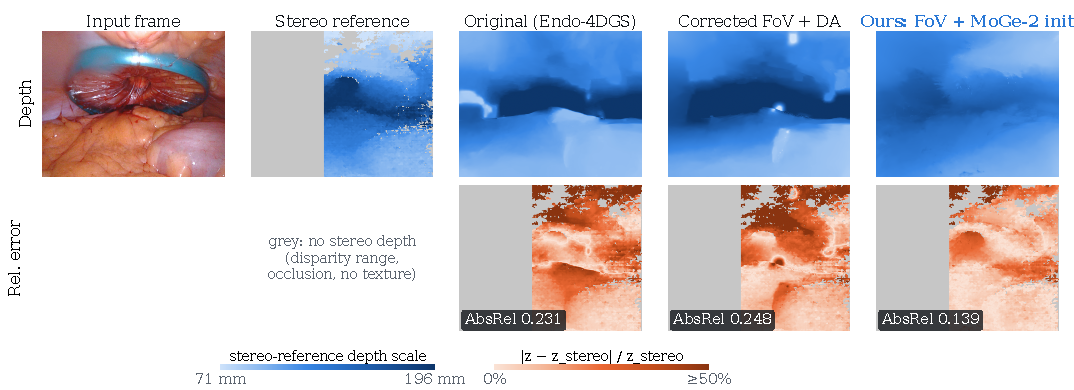
\includegraphics[width=\textwidth]{fig/qualitative.pdf}
\caption{Qualitative comparison on test frame 898 (median-error seed of each setup). Top: rendered depth on a shared scale; bottom: relative error against stereo depth. Correcting the field of view alone leaves the Depth-Anything geometry unchanged; MoGe-2 initialisation removes the spurious depth step below the instrument ring and lowers AbsRel from 0.231 to 0.139.}
\label{fig:qual}
\end{figure*}

\section{Method}
\textbf{Baseline.} Endo-4DGS back-projects the prior depth of the first frame into the initial point cloud and optimises colour, depth, depth-gradient, pseudo-normal and uncertainty losses (2k coarse + 6k fine iterations). The depth loss compares max-normalised maps and is scale invariant; the initialisation is not.

\textbf{Intrinsics.} The StereoMIS pose file stores the full-resolution, unrectified focal length (1039.6\,px), but the images are rectified and halved to 640$\times$512, which needs $f{=}569.0$\,px. Writing the rectified value changes the rendered horizontal field of view from 34.2$^\circ$ to 58.7$^\circ$.

\textbf{MoGe-2 prior and scale.} MoGe-2 (ViT-L) predicts a metric point map; we pass it the known field of view and store depth in mm, the unit of the poses. Its metric scale does not transfer to endoscopy: tissue is placed at $\sim$0.8\,m where stereo measures $\sim$0.12\,m. We recover one global scale from the poses alone: SIFT matches between frame pairs with $\geq$4\,mm baseline are triangulated with the known poses and
\begin{equation}
s=\operatorname{median}\left(z_{\text{tri}}/z_{\text{MoGe}}\right)=0.093
\end{equation}
(144 pairs, IQR 0.085--0.107). A stereo fit gives 0.165; the gap reflects kinematic pose error (2--6\,px epipolar), yet the pose-consistent scale trains better.

\textbf{Init-only training.} Our final model uses the scaled MoGe-2 depth only for initialisation and sets the depth, depth-gradient, normal and depth-uncertainty weights to zero.

\textbf{Explored alternatives.} (a)~A cosine loss between camera-frame rendered normals and MoGe-2 normals; (b)~COLMAP~\cite{colmap} bundle adjustment (BA) of the robot poses with fixed intrinsics, raw or with a temporally smoothed correction ($\sigma{=}15$ frames).

\section{Experimental Setup}
\textbf{Data and metrics.} StereoMIS P1, frames 801--1000 (left rectified view); every 8th frame (25) is a test view, 175 train. We report PSNR, SSIM and LPIPS, and for geometry compute reference depth by semi-global matching~\cite{sgm} on the stereo pair ($z{=}fb/d$, $fb{=}2494.6$\,px$\cdot$mm). Each rendered depth map is scaled to it by its per-frame median ratio; AbsRel and $\delta{<}1.25$ use pixels with valid stereo ($\approx$50\,\%). Main configurations use seeds 0--2. Table~\ref{tab:hw} lists hardware, software and compute.

\begin{table}[t]
\caption{Hardware, software and compute cost.}
\label{tab:hw}
\centering
\resizebox{\columnwidth}{!}{%
\begin{tabular}{@{}llll@{}}
\toprule
\multicolumn{4}{@{}l}{\textbf{Hardware:} RTX 4060 Ti 16\,GB, i9-12900K (24 threads), 62\,GB RAM, Ubuntu 24.04} \\
\multicolumn{4}{@{}l}{\textbf{Software:} Py 3.8/PyTorch 2.0.0/CUDA 11.8 (Endo-4DGS); Py 3.10/PyTorch 2.4.1 (MoGe-2); COLMAP 4.2} \\
\midrule
Depth prior & Params & Device & Time / frame \\
Depth-Anything ViT-B/14 (ONNX) & 97\,M & CPU & 0.75\,s \\
MoGe-2 ViT-L (3.2\,GB peak) & 331\,M & GPU & 0.22\,s \\
\midrule
Trained model & Gaussians & Render & Train (8k it.) \\
Original~\cite{endo4dgs} & 330\,k & 38\,FPS & 16.0\,min \\
Corrected FoV + DA & 352\,k & 35\,FPS & 17.0\,min \\
Ours (FoV + MoGe-2 init) & 327\,k & 38\,FPS & 15.9\,min \\
\bottomrule
\end{tabular}}
\end{table}

\begin{table}[t]
\caption{Main results on StereoMIS P1 (mean $\pm$ sample s.d., 3 seeds). AbsRel and $\delta$: per-frame scale-aligned, against SGBM stereo; see Table~\ref{tab:metric} for metric and fixed-scale errors.}
\label{tab:main}
\centering
\resizebox{\columnwidth}{!}{%
\begin{tabular}{@{}lccccc@{}}
\toprule
Setup & PSNR$\uparrow$ & SSIM$\uparrow$ & LPIPS$\downarrow$ & AbsRel$\downarrow$ & $\delta{<}1.25\uparrow$ \\
\midrule
\textit{Reported~\cite{endo4dgs}$^\dagger$} & \textit{32.69} & \textit{0.850} & \textit{0.148} & -- & -- \\
Original, reproduced & 31.98\pmsd{.09} & 0.8515\pmsd{.0010} & 0.178\pmsd{.003} & 0.234\pmsd{.004} & 0.603\pmsd{.014} \\
+ FoV fix (DA) & 32.33\pmsd{.14} & 0.8536\pmsd{.0019} & 0.186\pmsd{.002} & 0.235\pmsd{.039} & 0.611\pmsd{.067} \\
+ FoV, DA init only$^\ddagger$ & 32.62\pmsd{.13} & 0.8598\pmsd{.0016} & 0.166\pmsd{.001} & 0.376\pmsd{.048} & 0.404\pmsd{.078} \\
+ FoV, MoGe-2 + depth loss & 31.87\pmsd{.13} & 0.8436\pmsd{.0017} & 0.216\pmsd{.004} & 0.155\pmsd{.003} & 0.778\pmsd{.008} \\
\rowcolor{ours!12} \textbf{Ours}: FoV, MoGe-2 init ($\times$0.093) & 32.40\pmsd{.10} & 0.8526\pmsd{.0013} & 0.189\pmsd{.002} & 0.148\pmsd{<.001} & 0.795\pmsd{.001} \\
Ours, held-out-clean scale ($\times$0.104) & 32.29\pmsd{.06} & 0.8506\pmsd{.0007} & 0.194\pmsd{<.001} & 0.147\pmsd{.001} & 0.799\pmsd{.003} \\

\bottomrule
\end{tabular}}\\[2pt]
\parbox{\columnwidth}{\raggedright\scriptsize $^\dagger$As printed in~\cite{endo4dgs} (arXiv v4, Table 2; frames 800--1000; Depth-Anything Small, the paper's loss weights). Our reproduction uses the released code (commit 39c6ce2; Depth-Anything ViT-B). $^\ddagger$Depth-related terms and image TV disabled, as for ours.}

\end{table}

\section{Results}
\textbf{Quantitative.} Fixing the field of view adds 0.35\,dB PSNR for DA but leaves its scale-aligned depth error unchanged (AbsRel 0.235 vs.\ 0.234, with a large seed spread of 0.039; Table~\ref{tab:main}). MoGe-2 with the default depth losses gives a much lower depth error (0.155) but 0.46\,dB lower PSNR than FoV-corrected DA. Removing the group of depth-related terms (Section~\ref{sec:objective}) recovers the PSNR: our model is 0.42\,dB above the reproduced baseline in PSNR (+0.37 to +0.45\,dB per seed) and reduces the scale-aligned AbsRel by 37\,\% relative to it (seed s.d.\ 0.0004), with an SSIM change of only $+0.001$ and a worse LPIPS (0.189 vs.\ 0.178). The improvement is therefore in PSNR and depth agreement, not in every appearance metric. Against FoV-corrected DA the PSNR difference is small (+0.07\,dB) and the gain is in depth agreement. The same objective change applied to DA gives the highest PSNR (32.62\,dB) but a 61\,\% larger scale-aligned depth error than the reproduced baseline (0.376 vs.\ 0.234; 154\,\% larger than ours), so a better image metric does not imply better depth agreement (Fig.~\ref{fig:trade}). With the scale factor re-estimated from training frames only and filtered for consistency with the known poses ($\times$0.104; Section~\ref{sec:scale}), the model reaches 32.29\,dB and 0.147 AbsRel, i.e.\ the same depth agreement and a 0.11\,dB smaller PSNR gain. Our model has the lowest error on all 25 test frames (Fig.~\ref{fig:perframe}) at comparable training time and rendering speed (Table~\ref{tab:hw}).

\textbf{Ablations} (Table~\ref{tab:abl}). Each block varies one factor at the prior scale stated in the table. Raw MoGe-2 depth must be rescaled (29.51\,dB), and at matched FoV the pose-based scale gives higher PSNR than the stereo fit (31.87 vs.\ 31.56\,dB, 3 seeds vs.\ 1 seed). PSNR rises as the shared depth/gradient/TV weight $\lambda_d$ decreases, while the scale-aligned AbsRel stays at 0.148--0.159; disabling this group together with the normal and depth-uncertainty terms gives the best PSNR among the MoGe-2 variants. Because several terms are disabled jointly, this does not identify the effect of each term. Replacing the pseudo-normal loss by MoGe-2 normal supervision, compared at the same stereo-fitted scale, lowers PSNR by 0.12--0.28\,dB with AbsRel changes of at most 0.003. BA cuts long-baseline epipolar errors from up to 6.8 to $\sim$2\,px, but its per-frame poses jitter $\sim$10$\times$ more than the kinematic ones and cost about 2\,dB; a temporally smoothed correction still trails the robot poses, plausibly because rigid BA absorbs breathing motion (for MoGe-2 the prior scale also changes with the poses).

\begin{table}[t]
\caption{Ablations on P1 with corrected FoV (1 seed; $^\ast$3-seed mean). Each block varies one factor at the prior scale given in its first column; rows of different blocks are not directly comparable. AbsRel: per-frame scale-aligned, against stereo.}
\label{tab:abl}
\centering\scriptsize
\setlength{\tabcolsep}{3pt}
\begin{tabular}{@{}>{\raggedright}p{1.45cm}>{\raggedright}p{3.65cm}cc@{}}
\toprule
Factor & Variant & PSNR$\uparrow$ & AbsRel$\downarrow$ \\
\midrule
MoGe-2 scale & raw metric ($\times$1), 34.2$^\circ$ FoV & 29.51 & 0.186 \\
 & stereo-fitted ($\times$0.165), 34.2$^\circ$ FoV$^\ast$ & 31.09 & 0.162 \\
 & stereo-fitted ($\times$0.165), 58.7$^\circ$ FoV & 31.56 & 0.156 \\
 & pose-triangulated ($\times$0.093), 58.7$^\circ$ FoV$^\ast$ & 31.87 & 0.155 \\
\midrule
Depth weight $\lambda_d$ & 0.03 & 30.99 & 0.159 \\
(pose-scaled & 0.01 (default)$^\ast$ & 31.87 & 0.155 \\
MoGe-2, & 0.003 & 32.13 & 0.148 \\
$\times$0.093) & all depth terms and image TV off ($\lambda_d{=}\lambda_n{=}\lambda^{D}_{u}{=}0$)$^\ast$ & \best{32.40} & \best{0.148} \\
\midrule
Normal loss & reference: pseudo-normals, $w{=}0.001$ & 31.56 & 0.156 \\
(stereo-scaled & MoGe-2 normals, $w{=}0.01$ / $0.05$ & 31.44 / 31.28 & 0.155 / 0.153 \\
MoGe-2, $\times$0.165) & & & \\
\midrule
Poses$^\ddagger$ & raw BA: DA / MoGe-2 init & 29.97 / 30.73 & 0.292 / 0.149 \\
 & smoothed BA: DA / MoGe-2 init & 32.08 / 31.98 & 0.255 / 0.149 \\
 & robot poses: DA$^\ast$ / MoGe-2 init$^\ast$ & 32.33 / 32.40 & 0.235 / 0.148 \\
\bottomrule
\multicolumn{4}{@{}p{\columnwidth}@{}}{\scriptsize $^\ddagger$The MoGe-2 rows with BA poses re-estimate the prior scale from those poses ($\times$0.123 raw, $\times$0.124 smoothed), so pose and scale change together.}
\end{tabular}
\end{table}

\begin{figure}[t]
\centering
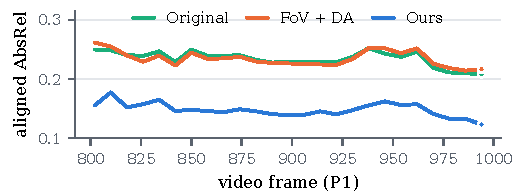
\includegraphics[width=\columnwidth]{fig/perframe.pdf}
\caption{Rendered-depth error per test frame (mean of 3 seeds).}
\label{fig:perframe}
\end{figure}

\begin{figure}[t]
\centering
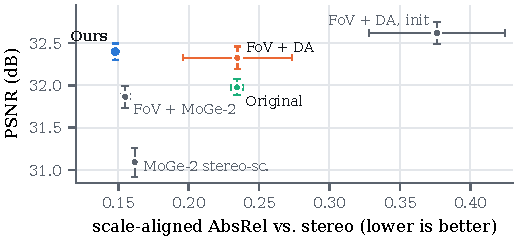
\includegraphics[width=\columnwidth]{fig/tradeoff.pdf}
\caption{Image quality vs.\ geometric accuracy, 3-seed means ($\pm$1 s.d.). Ours is the only setup better than the baseline on both.}
\label{fig:trade}
\end{figure}

\section{Conclusion}
A correct camera model and a properly scaled MoGe-2 initialisation improve Endo-4DGS in both image quality and 3D accuracy at no runtime cost; extra depth or normal supervision trades image quality for little geometric gain. Limitations: one 200-frame StereoMIS clip, stereo depth on about half of each frame, and no EndoNeRF data.

\begin{thebibliography}{9}
\scriptsize
\setlength{\itemsep}{0pt}
\bibitem{endo4dgs} Y.~Huang, B.~Cui, L.~Bai, Z.~Guo, M.~Xu, M.~Islam, and H.~Ren, ``Endo-4DGS: Endoscopic monocular scene reconstruction with 4D Gaussian splatting,'' in \emph{Proc. MICCAI}, 2024, pp.~197--207.
\bibitem{moge2} R.~Wang \emph{et al.}, ``MoGe-2: Accurate monocular geometry with metric scale and sharp details,'' arXiv preprint, 2025.
\bibitem{depthanything} L.~Yang, B.~Kang, Z.~Huang, X.~Xu, J.~Feng, and H.~Zhao, ``Depth Anything: Unleashing the power of large-scale unlabeled data,'' in \emph{Proc. CVPR}, 2024.
\bibitem{stereomis} M.~Hayoz \emph{et al.}, ``Learning how to robustly estimate camera pose in endoscopic videos,'' \emph{Int. J. Comput. Assist. Radiol. Surg.}, 2023.
\bibitem{kerbl3dgs} B.~Kerbl, G.~Kopanas, T.~Leimk\"uhler, and G.~Drettakis, ``3D Gaussian splatting for real-time radiance field rendering,'' \emph{ACM Trans. Graph.}, vol.~42, no.~4, 2023.
\bibitem{wu4dgs} G.~Wu \emph{et al.}, ``4D Gaussian splatting for real-time dynamic scene rendering,'' in \emph{Proc. CVPR}, 2024.
\bibitem{colmap} J.~L. Sch\"onberger and J.-M. Frahm, ``Structure-from-motion revisited,'' in \emph{Proc. CVPR}, 2016.
\bibitem{sgm} H.~Hirschm\"uller, ``Stereo processing by semiglobal matching and mutual information,'' \emph{IEEE Trans. Pattern Anal. Mach. Intell.}, vol.~30, no.~2, pp.~328--341, 2008.
\end{thebibliography}

\end{document}
